\documentclass{article}
\usepackage{tikz}

\begin{document}

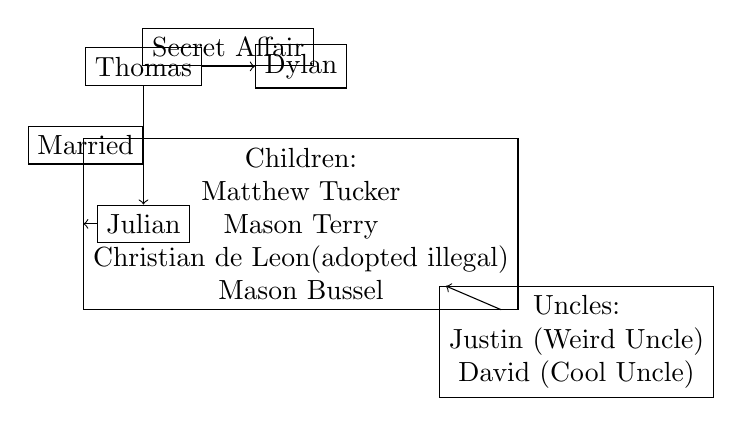
\begin{tikzpicture}[node distance=2cm, every node/.style={rectangle, draw, align=center}]
  % Nodes
  \node (thomas) {Thomas};
  \node [right of=thomas] (dylan) {Dylan};
  \node [below of=thomas] (julian) {Julian};
  \node [below of=dylan] (children) {Children:\\Matthew Tucker\\Mason Terry\\Christian de Leon(adopted illegal)\\Mason Bussel};
  \node [right of=children, xshift=1.5cm, yshift=-1.5cm] (uncles) {Uncles:\\Justin (Weird Uncle)\\David (Cool Uncle)};

  % Lines and arrows
  \draw[->] (thomas) -- (dylan) node[midway, above] {Secret Affair};
  \draw[->] (thomas) -- (julian) node[midway, left] {Married};
  \draw[->] (julian) -- (children);
  \draw[->] (children) -- (uncles);
\end{tikzpicture}

\end{document}